\begin{figure}[t]
\centering
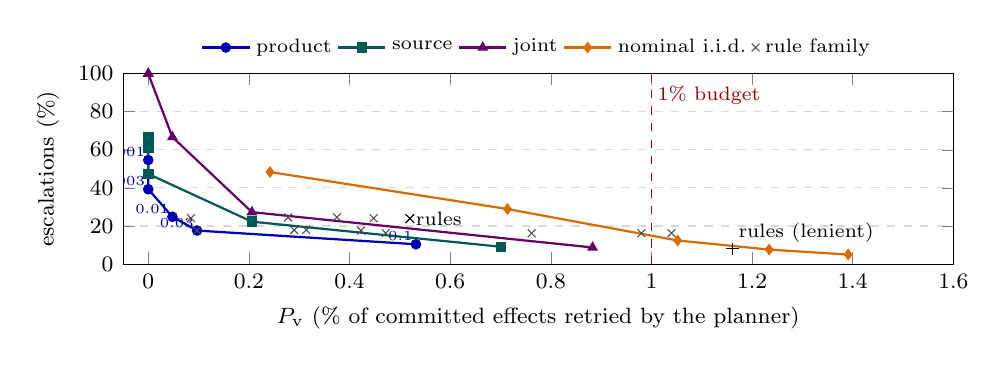
\begin{tikzpicture}
\begin{axis}[width=\linewidth,height=4.0cm,xlabel={$P_{\mathrm{v}}$ (\% of committed effects retried by the planner)},ylabel={escalations (\%)},
  xmin=-0.05,xmax=1.60,ymin=0,ymax=100,
  legend style={at={(0.5,1.03)},anchor=south,font=\scriptsize,draw=none,fill=none},legend columns=5,legend cell align=left,
  tick label style={font=\footnotesize},label style={font=\footnotesize},ymajorgrids,grid style={dashed,gray!30}]
\addplot[color=blue!70!black,mark=*,thick,mark size=1.5pt] coordinates {(0.532,10.42) (0.097,17.62) (0.048,24.85) (0.000,39.31) (0.000,54.68)};
\addlegendentry{product}
\addplot[color=teal!70!black,mark=square*,thick,mark size=1.5pt] coordinates {(0.701,9.10) (0.206,22.29) (0.000,47.35) (0.000,61.26) (0.000,66.70)};
\addlegendentry{source}
\addplot[color=violet!80!black,mark=triangle*,thick,mark size=1.5pt] coordinates {(0.883,8.73) (0.206,27.29) (0.048,66.72) (0.000,100.00) (0.000,100.00)};
\addlegendentry{joint}
\addplot[color=orange!85!black,mark=diamond*,thick,mark size=1.5pt] coordinates {(1.391,5.00) (1.234,7.64) (1.052,12.40) (0.714,28.92) (0.242,48.35)};
\addlegendentry{nominal i.i.d.}
\addplot[only marks,mark=x,mark size=2pt,gray!60!black] coordinates {(0.375,24.60) (0.980,16.21) (0.423,17.59) (0.448,24.09) (1.040,16.25) (0.314,17.97) (0.278,24.55) (0.762,16.20) (0.290,17.87) (0.085,24.15) (0.472,16.27) (0.097,17.62)};
\addlegendentry{rule family}
\addplot[only marks,mark=x,mark size=2.2pt,black,forget plot] coordinates {(0.520,23.90)};\node[font=\scriptsize,anchor=west,inner sep=2pt] at (axis cs:0.520,23.90) {rules};
\addplot[only marks,mark=+,mark size=2.2pt,black,forget plot] coordinates {(1.161,8.07)};\node[font=\scriptsize,anchor=south west,inner sep=2pt] at (axis cs:1.161,8.07) {rules (lenient)};
\node[font=\tiny,anchor=south east,inner sep=1pt,blue!60!black] at (axis cs:0.532,10.42) {0.1}; \node[font=\tiny,anchor=south east,inner sep=1pt,blue!60!black] at (axis cs:0.097,17.62) {0.03}; \node[font=\tiny,anchor=south east,inner sep=1pt,blue!60!black] at (axis cs:0.048,24.85) {0.01}; \node[font=\tiny,anchor=south east,inner sep=1pt,blue!60!black] at (axis cs:0.000,39.31) {0.003}; \node[font=\tiny,anchor=south east,inner sep=1pt,blue!60!black] at (axis cs:0.000,54.68) {0.001};
\draw[dashed,red!60!black] (axis cs:1,0) -- (axis cs:1,100) node[pos=0.97,anchor=north west,font=\scriptsize,inner sep=2pt] {1\% budget};
\end{axis}
\end{tikzpicture}\\[-1pt]
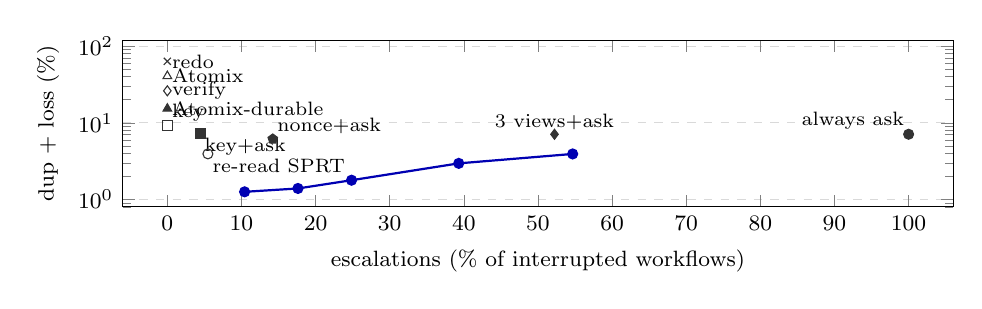
\begin{tikzpicture}
\begin{axis}[width=\linewidth,height=3.7cm,xlabel={escalations (\% of interrupted workflows)},ylabel={dup + loss (\%)},
  ymode=log,xmin=-6,xmax=106,ymin=0.8,ymax=120,log basis y=10,
  tick label style={font=\footnotesize},label style={font=\footnotesize},ymajorgrids,grid style={dashed,gray!30}]
\addplot[only marks,mark=x,mark size=1.8pt,gray!40!black] coordinates {(0.00,63.342)};\node[font=\scriptsize,anchor=west,inner sep=1.5pt] at (axis cs:0.00,63.342) {redo};
\addplot[only marks,mark=triangle,mark size=1.8pt,gray!40!black] coordinates {(0.00,40.675)};\node[font=\scriptsize,anchor=west,inner sep=1.5pt] at (axis cs:0.00,40.675) {Atomix};
\addplot[only marks,mark=triangle*,mark size=1.8pt,gray!40!black] coordinates {(0.00,15.300)};\node[font=\scriptsize,anchor=west,inner sep=1.5pt] at (axis cs:0.00,15.300) {Atomix-durable};
\addplot[only marks,mark=diamond,mark size=1.8pt,gray!40!black] coordinates {(0.00,26.125)};\node[font=\scriptsize,anchor=west,inner sep=1.5pt] at (axis cs:0.00,26.125) {verify};
\addplot[only marks,mark=square,mark size=1.8pt,gray!40!black] coordinates {(0.00,9.167)};\node[font=\scriptsize,anchor=south west,inner sep=1.5pt] at (axis cs:0.00,9.167) {key};
\addplot[only marks,mark=square*,mark size=1.8pt,gray!40!black] coordinates {(4.41,7.200)};\node[font=\scriptsize,anchor=north west,inner sep=1.5pt] at (axis cs:4.41,7.200) {key+ask};
\addplot[only marks,mark=pentagon*,mark size=1.8pt,gray!40!black] coordinates {(14.22,6.158)};\node[font=\scriptsize,anchor=south west,inner sep=1.5pt] at (axis cs:14.22,6.158) {nonce+ask};
\addplot[only marks,mark=diamond*,mark size=1.8pt,gray!40!black] coordinates {(52.23,7.083)};\node[font=\scriptsize,anchor=south,inner sep=1.5pt] at (axis cs:52.23,7.083) {3 views+ask};
\addplot[only marks,mark=otimes*,mark size=1.8pt,gray!40!black] coordinates {(100.00,7.092)};\node[font=\scriptsize,anchor=south east,inner sep=1.5pt] at (axis cs:100.00,7.092) {always ask};
\addplot[only marks,mark=o,mark size=1.8pt,gray!40!black] coordinates {(5.47,3.933)};\node[font=\scriptsize,anchor=north west,inner sep=1.5pt] at (axis cs:5.47,3.933) {re-read SPRT};
\addplot[color=blue!70!black,mark=*,thick,mark size=1.6pt] coordinates {(10.42,1.258) (17.62,1.392) (24.85,1.783) (39.31,2.958) (54.68,3.925)};
\end{axis}
\end{tikzpicture}
\caption{Top: escalations against the guaranteed quantity $P_{\mathrm{v}}$ as $\alpha{=}\beta$ sweeps from $0.1$ to $10^{-3}$ (labels on the product curve), against
the same-evidence rule family (wait 5/10/30/60\,s $\times$ quorum all / all but VLM / any two; gray $\times$), which has no guarantee; neither does a planner run at nominal $\alpha{=}0.1$. Bottom: total errors (including wrong user answers) against escalations; gray: baselines at their single operating point, blue: product sweep. Model-based simulation, default world.}
\label{fig:pareto}
\end{figure}
